\documentclass{beamer}
\usetheme{Berlin}
\usecolortheme{beaver}
\usepackage{graphicx}
\usepackage[export]{adjustbox}
\usepackage{tikz}
\usetikzlibrary{arrows}
\usepackage{amsmath}
\usepackage{lmodern}% http://ctan.org/pkg/lm
\usepackage{mathtools}
\usefonttheme{professionalfonts}

\title{Appendix: noise}
\subtitle{}
\author[Riccardo \and Eren]{Riccardo~Miccini\inst{1} \and Eren~Can~\inst{1}}
\institute[DTU]
{
	\inst{1}
	Technical University of Denmark\\
	Digital Communication
}
\date{\today}
\subject{Digital Communication}

\tikzstyle{int}=[draw, fill=blue!20]
\tikzstyle{every node}=[font=\tiny]

\begin{document}
\frame{\titlepage}

% ch A.2
\begin{frame}
	\frametitle{Characterization of noise in systems}
	\begin{itemize}
		\item Noise can be modeled and characterized on a subsystem-basis
		\item Each subsystem can be analyzed separately and optimized for low noise performances
	\end{itemize}
	\begin{figure}
		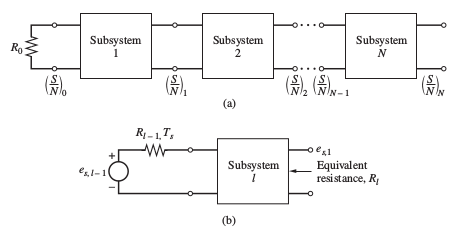
\includegraphics[width=0.8\textwidth]{subsys.png}
	\end{figure}
\end{frame}


% ch A.2.1
\begin{frame}
	\frametitle{Noise Figure of a System}
	\begin{itemize}
		\item Noise figure $F_l$: ratio between SNR at subsystem input and output: $ \left(\frac{S}{N}\right)_l = \frac{1}{F_l} \left(\frac{S}{N}\right)_{l-1} $
		\item Ideally, $ F_l = 1 $ (no additional noise introduced), tipically between 2 and 8 $dB$
		\item Without having to calculate the signal power: $ F_l = 1 + \frac{P_{int,l}}{G_a k T_0 B} $
		\begin{description}
			\item[$P_{int,l}$] Available, internally-generated noise power
			\item[$G_a$] Available power gain
			\item[$k$] Boltzmann's constant
			\item[$T_0$] Standardized temperature, $290 K$
			\item[$B$] Frequency band
		\end{description}
		\item For high gains, $F_l$ approaches 1
	\end{itemize}
\end{frame}


% ch A.2.3
\begin{frame}
	\frametitle{Noise Temperature}
	\begin{itemize}
		\item Power produced by a noisy resistor: $ P_{a,R} = kTB $
		\begin{description}
			\item[$k$] Boltzmann's constant, $ 1.38 \times 10^{-23} J/K $
			\item[$T$] Temperature of the resistor, in Kelvin
			\item[$B$] Frequency band, in Hertz
			\item[] Noise power independent on the resistor value
		\end{description}
		\item Equivalent noise temperature: $ T_n = \frac{P_{n,max}}{kB} $
	\end{itemize}
\end{frame}


% ch A.3
\begin{frame}
	\frametitle{Free Space Propagation Example}
	\begin{itemize}
		\item As a final work for the noise calculation, we will investigate the "free-space electromagnetic-wave propagation channel.
		\item To understand it fully on a practical example, we will investigate the communication tie between a synchronous-orbit relay satellite and a low-orbit satellite.
	\end{itemize}
\end{frame}


% ch A.3
\begin{frame}
	\frametitle{Free Space Propagation Example}
	\begin{itemize}
		\item As a final work for the noise calculation, we will investigate the "free-space electromagnetic-wave propagation channel.
		\item To understand it fully on a practical example, we will investigate the communication tie between a synchronous-orbit relay satellite and a low-orbit satellite.
	\end{itemize}
	\begin{figure}
		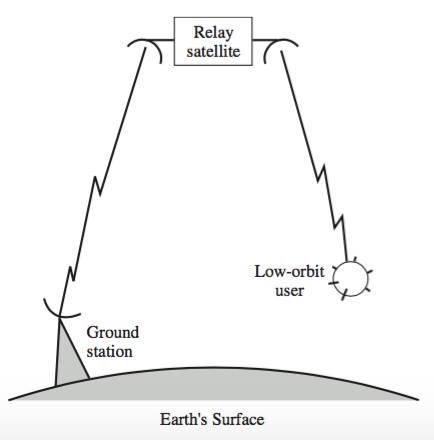
\includegraphics[width=0.35\textwidth]{orbit.png}
	\end{figure}
\end{frame}

\begin{frame}
	\frametitle{Investigating the Free-Space Propagation Example}
	\begin{itemize}
		\item We made some assumptions in regard to the example.
		\begin{enumerate}
			\item We have assumed that relay satellite transmitted signal power $P_t$
			\item It radiated isotropically
		\end{enumerate}
		\item Power density at a distance will be given by; $P_t=\frac{ P_t}{4 \pi d^2} W/m^2$
		\item If the satellite antenna has directivity, with the radiated power being directed toward low-orbit vehicle, antenna can be explained by the antenna power gain $G_T$ over the isotropic radiation level.
	\end{itemize}
\end{frame}

\begin{frame}
	\frametitle{Aperture-Type Antennas with Aperture Area $A_t$}
	\begin{itemize}
		\item For aperture-type antennas with aperture area $A_T$ large compared with the square of the transmitted wavelength $\lambda^2$.
		\item We can show that maximum gain will become:
		\begin{enumerate}
			\item $G_T= \frac{4 \pi A_T}{\lambda^2}$
			\item Also the power $P_R$ intercepted by the receiving antenna is given by the product of the receiving aperture area $A_R$ and the power density at the aperture. Thi will give us:
			$p_R= p_t A_R = \frac{P_T G_T}{4 \pi d^2} A_R$
		\end{enumerate}
		\item If we also include other loses and use maximum gain $G_R$, it will yield into this formula: $P_R=(\frac {\lambda}{4 \pi d })^2  \frac{P_T G_T G_R}{L_0} $
		\item The factor $(\frac{4 \pi d}{\lambda})^2$ is referred as the "free-space loss"
	\end{itemize}
\end{frame}

\begin{frame}
	\frametitle{Receiver Power}
	\begin{itemize}
		\item It is easier to work with decibels when we calculate the receiver power.
		\item If we take the $10 \log_ {10}  P_R$, than we obtain :
		 $10 \log_{10} P_R= 20 \log_{10} (\frac{\lambda}{4 \pi d}) +  10 \log_{10} P_T+10 \log_{10} G_T+10 \log_{10} G_R - 10 \log_{10} L_0 $
		 \item $10 \log_{10} P_R $ can be interpreted as receiver power in decibels referenced to 1 $W$
		 \item Also $10 \log_{10} P_T$  is referred as the transmitted signal in $dbW$
	\end{itemize}
\end{frame}


\end{document}
